\section{Теоретическая часть}
\subsection{Основные определения и соотношения}
Одним из наиболее эффективных промышленных методов разделения изотопов 
лёгких элементов (водорода, лития, бора, углерода и др.) является 
физико-химический метод изотопного обмена. Важной особенностью 
физико-химических методов является обратимость элементарного акта разделения 
и двухфазность рабочей системы.

Наиболее удобной рабочей двухфазной системой считается система 
жидкость – газ. Процесс разделения изотопов при этом проводят в 
разделительных колоннах, при непрерывном противоточном движении потоков 
жидкой ($L$) и газовой ($G$) фаз. Поскольку значения констант равновесия, 
летучестей и т. д. для различных изотопнозамещенных форм различно, 
то возникает изотопный эффект, приводящий к изменению содержания данного 
изотопа в разных фазах. Вследствие этого эффекта, характеризуемого величиной 
коэффициента разделения $\alpha$, содержание изотопа в фазе $L$, покидающей 
некоторое сечение колонны II будет отличаться от содержания этого же изотопа 
в фазе $G$, покидающей сечение I:
\begin{equation}
\alpha = \dfrac{c_{2}(1-c_{1})}{c_{1}(1-c_{2})}
\end{equation}
\noindent где $c_{1}, c_{2}$ – мольные доли целевого изотопа в равновесных фазах.

Уравнение, описывающее обогащение в каскаде из элементов второго рода, 
при условии, что $\alpha$ для всех элементов одинаково, а коэффициент 
обогащения $\varepsilon = (\alpha – 1) << 1$ и поток отбора $P << L$ 
имеет вид:
\begin{equation}
\dfrac{dc}{dn} = \varepsilon c(1-c) - \dfrac{P}{L}(c_{P}-c)
\end{equation}
\noindent где $c_{P}$ – концентрация отбора.

\subsection{Принципиальная схема работы колонны или каскада колонн}
Разделительные колонны различаются по виду, особенностям строения и работы. 
На рисунке ~\ref{fig:cascade} приведена схема работы колонны.
\begin{figure}[hbtp]
    \centering
    \captionsetup{justification=centering}
    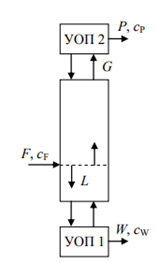
\includegraphics[scale=1]{latex/figures/figure1.png}
    \caption{Схема процесса разделения изотопов}
    Обозначения: $c_{P}$, $c_{F}$, $c_{W}$ – концентрации отбора, питания, отвала;
    
    $P$, $F$, $W$ – потоки отбора, питания, отвала
    \label{fig:cascade}
\end{figure}

Разделяемая бинарная смесь изотопов подаётся в среднюю часть колонны 
(рисунок ~\ref{fig:cascade}), в которой осуществляется противоточное движение фаз. 
Проходя последовательно ряд разделительных элементов, одна из фаз обогащается 
лёгким изотопом, а другая – тяжёлым. На концах колонны имеются специальные 
аппараты, которые предназначены для создания противоточного движения 
фаз путём перевода смеси изотопов из одной фазы в другую.

В стационарном режиме работы колонны справедливы следующие соотношения 
материального баланса:
\begin{equation}
    Fc_{F} = Pc_{P} + Wc_{W}
\end{equation}
\begin{equation}
    F = P + W
\end{equation}

В ряде случаев при большой высоте колонны и, исходя из различных практических 
особенностей организации разделительного процесса, колонну разбивают на 
несколько, образующие каскад колонн.
\newpage